% Assign classrooms

Let the set $S$ contain as elements number of students in each course $i$ (denote $s_i$) and set $C$ contain as elements number of chairs in each classroom $j$ (denote $c_j$). We now sort both the sets $S$ and $C$ in ascending order. Since we are trying to minimize the ``disparity" measure ($|s - c|$) over all the assignments, once these sorted numbers are put in a number line the optimal assignment looks like follows: \\



% Define style for nodes
\tikzstyle{every node}=[circle, draw, fill=black!50,
                        inner sep=0pt, minimum width=4pt]
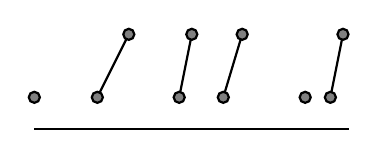
\begin{tikzpicture}[thick,scale=0.8]
  \draw (0,0) node {};
    \draw (1,0) node {} --  (1.5,1) node {};
    \draw (2.3,0) node {} --  (2.5,1) node {};
    \draw (3,0) node {} --  (3.3,1) node {};
    \draw (4.3,0) node {};
    \draw (4.7,0) node {} --  (4.9,1) node {};
    \draw (0, -0.5) -- (5, -0.5);

    
\end{tikzpicture}\quad



We can observe that under optimal assignment the lines assigning courses to classrooms do not cross each other, else it would not be an optimal assignment. In other words, for course $i$ and $j$ with $s_i < s_j$, course $i$ is never assigned a classroom bigger than the one assigned to course $j$. This observation allows us to define subproblems to the original problem in an easy way.

In the following, we introduce two algorithms, one runs in $O(mn^2)$, one in $O(mn)$.

\section{$O(mn^2)$ Algorithm}

We define $OPT(n', m')$ as the optimal assignment (one that minimizes the cost function) for a sub-problem containing $n'$ courses and $m'$ classrooms where $m' \geq n'$.



Since all courses need to be assigned a classroom, when the arrays are sorted course $n'$ can only be assigned one of the classes with indices in the interval $[n', m']$.

Now the recurrence relation for the subproblem can be formulated as :

\begin{center}
  $OPT(n', m') = \min\limits_{n'\leq k \leq m'} (OPT(n'-1, k-1) + |s_{n'} - c_{k}|)$
\end{center}

So we need to maintain a table of size $mn$ to find the optimal solution to the original problem, and to fill each entry in the table requires $O(m)$, hence the  complexity $O(mn^2)$.

\section{$O(mn)$ Algorithm}

We assume the classrooms and courses are sorted in ascending order. Now we turn this problem into a \textit{Global Sequence Alignment} problem, with following definition of cost:

\[
\begin{array}{l l l}
  \text{Cost(insertion of room $c_i$)} & = & 0 \\
  \text{Cost(insertion of course $s_i$)} & = & \infty \\
  \text{Cost(matching course $s_i$ with room $c_j$)} & = & |s_i - c_j|
\end{array}
\]

As we know the standard \textit{Global Sequence Alignment} runs in $O(mn)$, so the optimal matching takes $O(mn)$. The matching pairs can be found using backward tracking from entry $(s_n, c_m)$ to $(s_1, c_1)$. Each diagonal arrow in the backward path is a matching pair. The backward tracking takes $O(m + n)$.